\documentclass[11pt]{amsart}
%%%%%%%%%%%%%% Packages
\usepackage{amssymb,amsfonts,amsthm,amsmath}
\usepackage[english]{babel}
\usepackage[all,cmtip]{xy}
\usepackage{tikz}
\usepackage{mathtools}
\usepackage{tensor}
\usepackage{csquotes}
\usepackage[vcentermath]{youngtab}
%\usepackage{stix}
\usetikzlibrary{arrows,chains,matrix,positioning,scopes}
%\usepackage{mathrsfs}
%\usepackage[notcite,notref]{showkeys}


%%%%%%%%%%% Tikz
\makeatletter
\tikzset{join/.code=\tikzset{after node path={%
\ifx\tikzchainprevious\pgfutil@empty\else(\tikzchainprevious)%
edge[every join]#1(\tikzchaincurrent)\fi}}}
\makeatother
\tikzset{>=stealth',every on chain/.append style={join},
         every join/.style={->}}

        

%%%%%%%%%%%% Personalized commands and environments

\newcommand{\inputc}[1]{ \raisebox{-0.5\height}{\input{#1}} }
\newtheorem{theorem}{Theorem}
\newtheorem{lemma}[theorem]{Lemma}
\newtheorem{corollary}[theorem]{Corollary}
\newtheorem{definition}[theorem]{Definition}
\newtheorem{proposition}[theorem]{Proposition}
\newtheorem{remark}[theorem]{Remark}
\newtheorem{example}{Example}
%\newtheorem{theorem*}{Theorem}

\newcommand{\func}[3]{{#1} : {#2} \longrightarrow {#3}}
\numberwithin{equation}{section}
\newcommand{\dbar}{\bar{\partial}}
\newenvironment{myproof}{\noindent{it Proof}
\setlength{\parindent}{0mm}}
{$\hfill \bs$}


%%%%%%%%%%%%%%%%%%%%%%%% Title and Author information

\title{MAT 303 Recitations: Week 11}


\author[M. Gomes]{Marlon de Oliveira Gomes}
\address{Mathematics Department 3-101, Stony Brook University,
100 Nicolls Road, Math Tower, 
Stony Brook, NY, 11794, USA} \email{mgomes@math.stonybrook.edu}



%%%%%%%%%%% Text
\begin{document}

\maketitle


\section*{Section 3.4: Mechanical Vibrations}

In this section we deal with second-order differential equations of type
\begin{equation*}
mx''(t)+cx'(t)+kx(t) = F(t),
\end{equation*}
where $m,c,k$ are positive constants which denote the mass, the damping constant, and the spring constant in the context of a mass-spring-dashpot system, respectively. General solutions to such equations take the form 
\begin{equation*}
x(t)=x_c(t)+x_p(t)
\end{equation*}
where $x_c$ is a complementary solution to the associated homogeneous problem, and $x_p$ is a particular solution to the equation. 

The first few homework problems deal with homogeneous equations. We learned how to express solutions as combinations of sines, cosines, and exponentials in the last couple of weeks, but now we adopt a slightly different convention regarding trigonometric representations. We will write 
\begin{equation*}
A\cos(\omega_1 t)+ B \sin(\omega_1 t) = C\cos(\omega_1 t -\alpha),
\end{equation*}
where 
\begin{itemize}
\item $C=\sqrt{A^2+B^2}$ is the amplitude; 
\item $\alpha \in [0, 2\pi)$ is the phase, so that $\cos(\alpha)=\frac{A}{C}$ and $\sin(\alpha)=\frac{B}{C}$.
\end{itemize} 

\begin{example}
Problem 3.4.4 concerns the movement of a mass-spring system, with:
\begin{itemize}
\item $m=250g=0.25kg$;
\item $k=9N/0.25m = 36N/m$;
\end{itemize}
and initial conditions $x(0)=1m, x'(0)=-5m/s$.

The movement of the system is described by the equation
\begin{equation*}
0.25x^{''}+36x=0 \Leftrightarrow x^{''}+144x=0,
\end{equation*}
thus the relative frequency is $\omega=12$. A solution can be written in form
\begin{equation*}
x(t)=C\cos(12t-\alpha),
\end{equation*}
for constants $C>0$, $\alpha\in [0,2\pi)$ to be determined.

Finding these constants amounts to using the initial conditions. From $x(0)=1$, $x'(0)=-5$, we obtain
\begin{equation*}
C\cos(\alpha)  =1, \  C\sin(\alpha)  = -\frac{5}{12},
\end{equation*}
thus $C=\sqrt{1+\left(\frac{5}{12}\right)^2}=\frac{13}{12}$. The value of $\alpha$ (in radians) that satisfies the constraints above is found by calculator:
\begin{equation*}
\alpha \approx 5.89.
\end{equation*}
Thus 
\begin{equation*}
x(t)\approx \frac{13}{12}\cos(12t-5.89),
\end{equation*}
from which we infer the amplitude
\begin{equation*}
A=\frac{13}{12}m,
\end{equation*}
and the period
\begin{equation*}
T=\frac{2\pi}{12}=\frac{\pi}{6}s.
\end{equation*}
\end{example}

\begin{example}
In problem 3.4.14, we have a mass-spring-dashpot system with constants
\begin{equation*}
m=25, c=10, k=226,
\end{equation*}
and initial data $x(0)=20, x'(0)=41$. Its characteristic polynomial is 
\begin{equation*}
25r^2+10r+226 = (5r+1)^2+15^2, 
\end{equation*}
whose roots are 
\begin{equation*}
r=-\frac{1}{5}\pm 3i.
\end{equation*}
Solutions to the differential equation take the form
\begin{equation*}
x(t)=Ce^{-\frac{t}{5}}\cos(3t-\alpha).
\end{equation*}
To use the initial data, we compute the first derivative,
\begin{equation*}
x'(t)=-Ce^{-\frac{t}{5}}\left[\frac{\cos(3t-\alpha)}{5}+3\sin(3t-\alpha)\right],
\end{equation*}
hence (using parity properties of the cosine and sine functions)
\begin{align*}
C\cos(\alpha) & = 20 \\
C\left[ - \frac{\cos(\alpha)}{5} + 3\sin(\alpha) \right] & = 41,
\end{align*}
from which we infer $C=25$, $\alpha \approx 0.64$, so 
\begin{equation*}
x(t) \approx 25e^{-\frac{t}{5}}\cos(3t-0.64).
\end{equation*}
\end{example}

\begin{example}
In problem 3.4.17, we are meant to contrast the damped motion of a spring-mass-dashpot system with its undamped counterpart. The differential equation modelling this problem is
\begin{equation*}
x^{''}+8x^{'}+16x=0,
\end{equation*}
 with initial data $x(0)=5, x'(0)=-10$. The characteristic polynomial of the problem is 
\begin{equation*}
r^2+8r+16=(r+4)^2.
\end{equation*}
Its root is $-4$, with multiplicity 2, thus this motion is critically damped. 

A general 
solution takes the form 
\begin{equation*}
    x(t)=e^{-4t}(At+B), 
\end{equation*}
and has derivative
\begin{equation*}
x'(t) = e^{-4t}(-4At+A-4B).
\end{equation*}
Subject to initial conditions $x(0)=5, x'(0)=-10$, we find 
\begin{equation*}
x(t)=5e^{-4t}(2t+1).
\end{equation*}

The equation that models undamped motion is 
\begin{equation*}
u^{''}(t)+16u(t) = 0.
\end{equation*}
Its solutions take the form 
\begin{equation*}
u(t)=C\cos(4t-\alpha).
\end{equation*}
Assuming the same initial conditions $u(0)=5, u'(0)=-10$, we have 
\begin{equation*}
u(t)\approx \frac{5\sqrt{5}}{2}\cos(4t-5.82)
\end{equation*}

\begin{center}
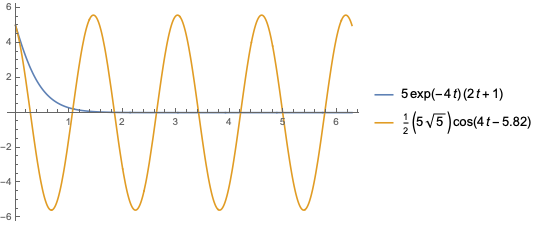
\includegraphics[width=0.8\textwidth]{p2.png}
\end{center}

\end{example}

\begin{example}
In problem 3.4.31, we have a mass-spring-dashpot system with constants $m=1, c=10$ and $k=125$, subject to initial conditions $x(0)=6$, $x'(0)=50$. The characteristic polynomial of the system is 
\begin{equation*}
r^2+10r+125 = (r+5)^2+10^2,
\end{equation*}
whose roots are $r=-5 \pm 10i$, characterizing underdamped motion. The corresponding solution to the diferential equation is 
\begin{equation*}
x(t)=Ce^{-5t}\cos(10t-\alpha),
\end{equation*}
for constants $C>0$, $\alpha \in [0,2\pi)$ to be determined in what follows.
 
The first derivative of the solution takes the form
\begin{equation*}
x^{'}(t)  = Ce^{-5t}[-5\cos(10t-\alpha)-10\sin(10t-\alpha)].
\end{equation*}
The initial conditions amount to
\begin{align*}
C\cos(\alpha) & =6, \\
C[-10\cos(\alpha)-5\sin(\alpha)] & = 50,
\end{align*}
from which we infer $C=10$, $\alpha\approx 0.93$. The solution is thus approximated by
\begin{equation*}
x(t)\approx 10e^{-5t}\cos(10t-0.93).
\end{equation*}

We will constrast this to solutions of the undamped motion, modelled by the equation
\begin{equation*}
u''+125u=0.
\end{equation*}
The characteristic polynomial is $p(r)=r^2+125$, with roots $r=\pm5\sqrt{5}i$. Solutions to this equation can be expressed as
\begin{equation*}
u(t)=C_{*}\cos(5\sqrt{5}t-\alpha_{*}),
\end{equation*}
where the constants $C_{*}>0$ and $\alpha_{*} \in [0, 2\pi)$ are determined by the initial conditions $u(0)=6, u'(0)=50$. The derivative of a solution takes the form 
\begin{equation*}
u'(t)=-5\sqrt{5}C_{*}\sin(5\sqrt{5}t-\alpha_{*}), 
\end{equation*}
so using the initial date we obtain 
\begin{align*}
C\cos(\alpha_{*}) & =6  \\
5\sqrt{5}C_{*}\sin(\alpha_{*}) & = 50,
\end{align*}
and infer $C_{*} = 2\sqrt{14}$, $\alpha_{*} \approx 0.64$. Finally, we motion of the undamped system is 
\begin{equation*}
u(t)  \approx 2\sqrt{14}\cos(5\sqrt{5}t-0.64).
\end{equation*}

Below is a graphical comparison between the motions of the damped and undamped system
\begin{center}
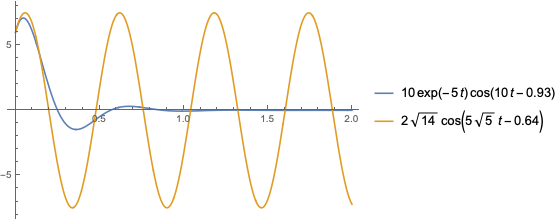
\includegraphics[width=0.8\textwidth]{p1.png}
\end{center}
\end{example}


\section*{Section 3.5: Nonhomogeneous Equations and Undetermined Coefficients}

The method of undetermined coefficients deals with nonhomogeneous equations with constant coefficients. 

\begin{example}
In problem 3.5.3, we consider the equation 
\begin{equation}\label{3.5.3}
y^{''}-y^{'}-6y=2\sin(3x).
\end{equation}
The associated homogeneous equation has characteristic polynomial
\begin{equation*}
r^2-r-6=(r+2)(r-3),
\end{equation*}
with roots $r_1=-2, r_2=3$. The corresponding solutions to the complementary equation take the form 
\begin{equation*}
y_c=A_1e^{-2x}+A_2e^{3x}.
\end{equation*}
As the solutions to the homogeneous problem and the inhomogeneous term of equation \eqref{3.5.3} are linearly independent (verify!), we can use the method of undetermined coefficients to guess a particular solution of the form 
\begin{equation*}
y_p=C_1\sin(3x)+C_2\cos(3x).
\end{equation*}
To find the coefficients $C_1,C_2$, we need to compute the derivatives of the particular solution, 
\begin{align*}
y_{p}^{'} & = 3C_1\cos(3x)-3C_2\sin(3x), \\
y_{p}^{''} & = -9C_1\sin(3x)-9C_2\cos(3x).
\end{align*}
Combining all of this data into the equation we get
\begin{equation*}
(-15C_1+3C_2)\sin(3x) + (-3C_1-15C_2)\cos(3x) = 2\sin(3x), 
\end{equation*}
from which we infer $C_1=-\frac{5}{39}$, $C_2=\frac{1}{39}$. A general solution to the differential equation takes the form
\begin{equation*}
y(x)=A_1e^{-2x}+A_2e^{3x}-\frac{5}{39}\sin(3x)+\frac{1}{39}\cos(3x),
\end{equation*}
for constants $A_1$ and $A_2$ to be determined based upon initial conditions. 
\end{example}

\begin{example}
In problem 3.5.10 we have a case of duplication, the inhomogeneous term is linearly dependent with the complementary solutions. The equation in question is 
\begin{equation*}
y^{''}+9y=2\cos(3x)+3\sin(3x).
\end{equation*}
The characteristic polynomial of the equation is 
\begin{equation*}
r^2+9=(r+3i)(r-3i),
\end{equation*}
with roots $3i$ and $-3i$. The corresponding complementary solutions take the form
\begin{equation*}
y_c(x)=A_1\cos(3x)+A_2\sin(3x).
\end{equation*}
A guess of type 
\begin{equation*}
y(x)=C_1\cos(3x)+C_2\sin(3x)
\end{equation*}
would never solve the inhomogeneous problem, as it makes the left hand side of the equation vanish. To fix this, we introduce a monomial factor
\begin{equation}\label{3.5.10}
y_p(x)=C_1x\cos(3x)+C_2x\sin(3x).
\end{equation}
As we will see below, this will be enough for our purposes. A remark about the form of the solutions is in place. Adding extraneous terms of lower order, such as 
\begin{equation*}
C_1x\cos(3x)+C_2x\sin(3x)+C_3\cos(3x)+C_4\sin(3x)
\end{equation*}
is a waste of time, as the last two components satisfy the homogeneous problem. The complementary solution should only be added at the end of the problem, as you will see below. 

We will continue with the derivation of the particular solution \eqref{3.5.10}. Its derivatives are 
\begin{align*}
y_{p}^{'}(x) & = C_1\cos(3x)+C_2\sin(3x)-3C_1x\sin(3x)+3C_2x\cos(3x) \\
y_{p}^{''}(x)& = -6C_1\sin(3x) + 6C_2\cos(3x) -9C_1x\cos(3x)-9C_2x\sin(3x)
\end{align*}
Combining derivatives according to the equation we obtain
\begin{align*}
y_{p}^{''}+9y_p & = 2\cos(3x)+3\sin(3x) \\
 -6C_1\sin(3x)+6C_2\cos(3x) & = 2\cos(3x)+3\sin(3x),
\end{align*}
thus $C_1=-\frac{1}{2}$ and $C_2=\frac{1}{3}$. The final form of a general solution to the inhomogeneous problem is 
\begin{equation*}
y(x)=A_1\cos(3x)+A_2\sin(3x)-\frac{1}{2}x\cos(3x)+\frac{1}{3}x\sin(3x), 
\end{equation*}
for constants $A_1$, $A_2$ to be determined based upon initial conditions.
\end{example}
\begin{thebibliography}{0}

\bibitem{EdPeCa} C. Henry Edwards, David E. Penney and David T. Calvis, {\it Differential Equations and Boundary Value Problems: Computing and Modelling}, 5th edition, Pearson, 2014.

\end{thebibliography}
\end{document}


